\documentclass[aspectratio=1610]{beamer}
\title[Multi-modal RAG]
{Multi-modal Retrieval-Augmented Generation (RAG): \\
Tackling Hallucination in Multimodal Question Answering}
\author{LAM, Ching Yin}
\institute[CPEG4902, CSE, HKUST]
{DAN1 \\
Advised by Prof. Dan XU \\
CPEG 4902, 2025-2026 \vspace{2mm}\\
Department of Computer Science and Engineering \\
The Hong Kong University of Science and Technology}
\date{May 5, 2026}
\usefonttheme[onlymath]{serif}
\usetheme{CambridgeUS}
\usepackage{verbatim}
\usepackage{fancyvrb}
\usepackage{parskip}
\usepackage{graphicx}
\usepackage{booktabs}
\usepackage{ltablex}

\setbeamertemplate{navigation symbols}{}
\setlength{\parindent}{0pt}
\setlength{\parskip}{6pt}

\begin{document}
    \begin{frame}
        \titlepage
    \end{frame}

    \section{Introduction}
    \begin{frame}
        \frametitle{Outline}
        \tableofcontents[currentsection, subsectionstyle=show/shaded] 
    \end{frame}

    \begin{frame}
        \frametitle{Overview of RAG}
        \begin{itemize}
            \item Retrieval-Augmented Generation (RAG) has become the dominant method in grounding LLM generation with evidence
            \item Successful in text-only settings
        \end{itemize}

        \begin{figure}[H]
            \centering
            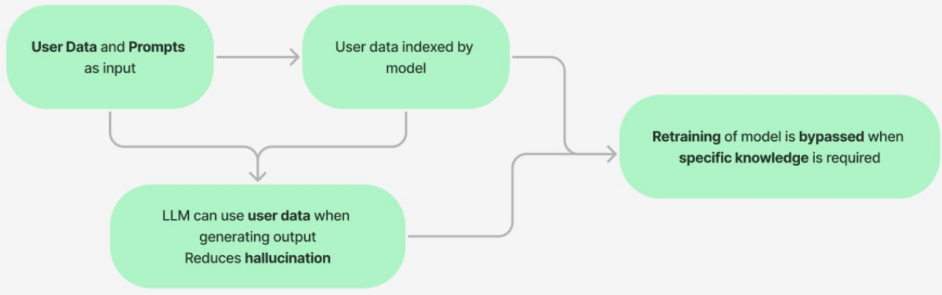
\includegraphics[width=0.8\textwidth]{images/1-intro/rag-rationale.png}
            \caption{How RAG benefits LLM generation}
        \end{figure}
    \end{frame}

    \begin{frame}
        \frametitle{Why Multimodal RAG?}
        Multimodal RAG can be useful in high-stakes domains and situations, such as
        \begin{itemize}
            \item a domain expert querying a MLLM on fine differences between rare bird species
            \item an engineer asking a MLLM about specific design elements in blueprints
            \item a doctor inspecting X-ray scans for certain diseases with MLLM assistance
        \end{itemize}
    \end{frame}

    \begin{frame}
        \frametitle{Problem and Objectives}
        The problems with current RAG pipelines are:
        \begin{itemize}
            \item Current text-only RAG pipelines do not apply to multimodal LLMs (MLLMs)
            \item Limitations in emerging multimodal RAG pipelines: \\
                    visual cues or fine details overlooked by visual encoders (such as CLIP) used
            \item Grounding with retrieved visual evidence remains challenging
        \end{itemize}

        This thesis is built on the following goals and hypothesis:
        \begin{itemize}
            \item \textbf{Hypothesis}: separate feature spaces for visual and text outperforms unified embeddings
            \item Preserve fine-grained visual features in visual evidence retrieval
            \item Use state-of-the-art specialized models to enable cross-modal retrieval without fine-tuning
        \end{itemize}
    \end{frame}

    \section{Methodology}
    \begin{frame}
        \frametitle{Outline}
        \tableofcontents[currentsection, subsectionstyle=show/shaded] 
    \end{frame}

    \begin{frame}
        \frametitle{High-Level Architecture}
        \begin{figure}[H]
            \centering
            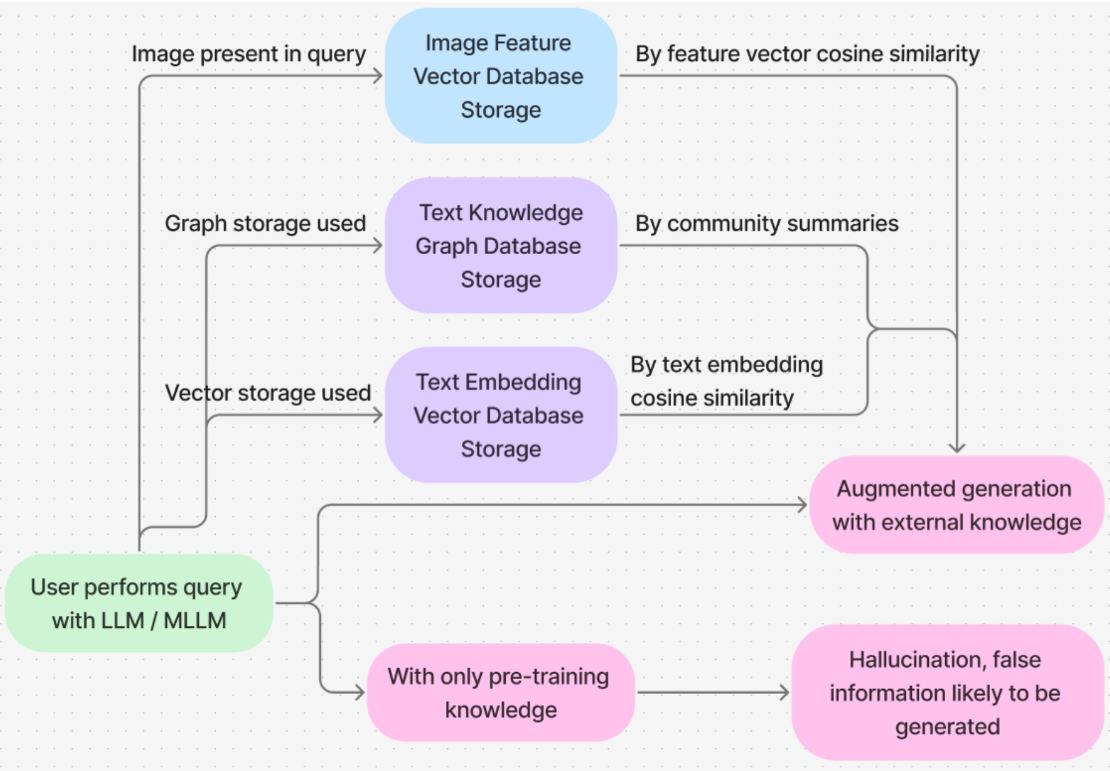
\includegraphics[width=0.65\textwidth]{images/2-method/high-level-overview.png}
            \caption{A high level overview of the entire project and implementation}
        \end{figure}
    \end{frame}

    \begin{frame}[fragile]
        \frametitle{Document Preprocessing}
        \begin{itemize}
            \item Split document text into fixed-sized overlapping text chunks
            \item Extract inline images and surrounding text context for captioning
            \item Replace images with their captions
        \end{itemize}

        \begin{figure}[H]
            \centering
            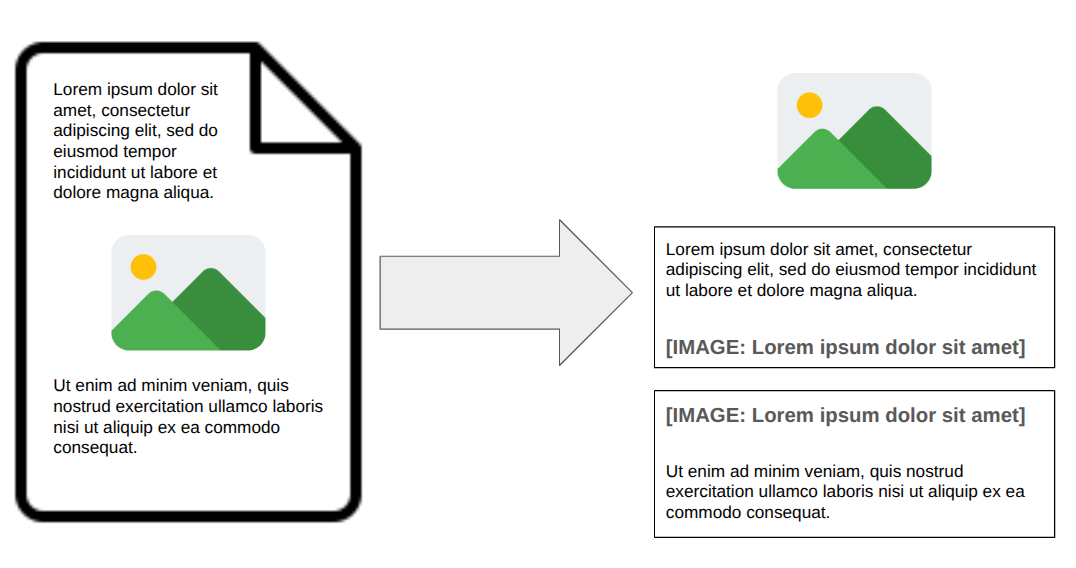
\includegraphics[width=0.58\textwidth]{images/2-method/parsing-concept.png}
            \caption{Our document parsing method}
        \end{figure}
    \end{frame}

    \begin{frame}[fragile]
        \frametitle{Embedding}
        We embed text and extracted images separately.

        \begin{figure}[H]
            \centering
            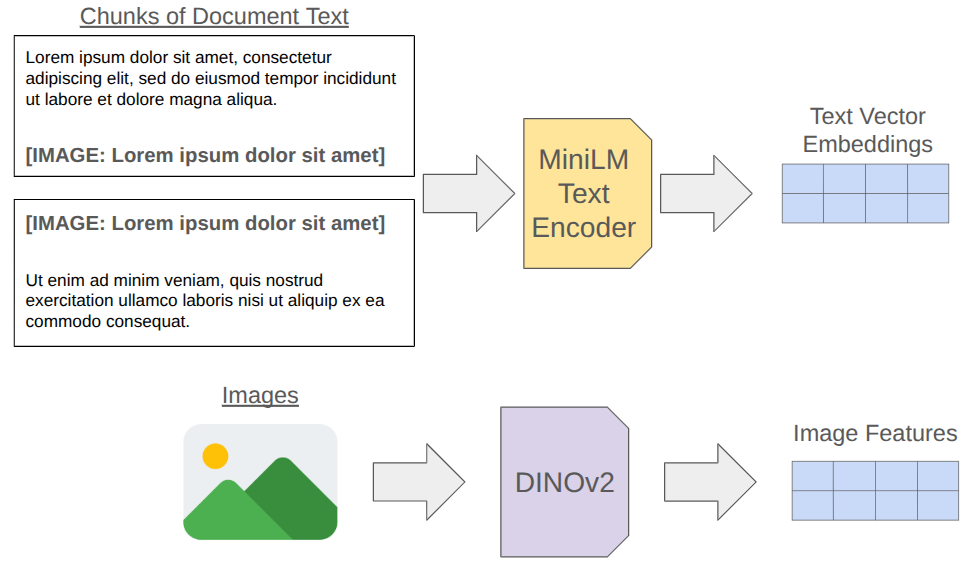
\includegraphics[width=0.6\textwidth]{images/2-method/embedding-concept.png}
            \caption{Embedding text and images into separate representations}
        \end{figure}
    \end{frame}

    \begin{frame}[fragile]
        \frametitle{Embedding}
        For \textbf{text},
        \begin{itemize}
            \item Map sentences or paragraphs into high-dimensional dense vector space
            \item Use MiniLM model (\verb|sentence-transformers/all-MiniLM-L6-v2|) to embed text chunks
        \end{itemize}

        For \textbf{images},
        \begin{itemize}
            \item Use DINOv2, a vision-specific model, to extract feature vectors
            \item Embed captions in the same way as text chunks
        \end{itemize}
    \end{frame}
    
    \begin{frame}
        \frametitle{Storage}
        We store text embedding vectors and image feature vectors separately.
        \begin{itemize}
            \item \textbf{Text embeddings} stored in a vector database
            \item \textbf{Image features} and \textbf{caption text embeddings} stored in a \emph{multi-vector} database
        \end{itemize}

        Alternately, we also experiment with knowledge graph storage.
        \begin{itemize}
            \item Extract \textbf{entities} and \textbf{relationships} with an LLM
            \item Entities form nodes, relationships form edges
            \item Detect communities with Louvain's Algorithm
            \item Generate community summary for each community
        \end{itemize}
    \end{frame}

    \begin{frame}
        \frametitle{Processing Flow}
        \begin{figure}[H]
            \centering
            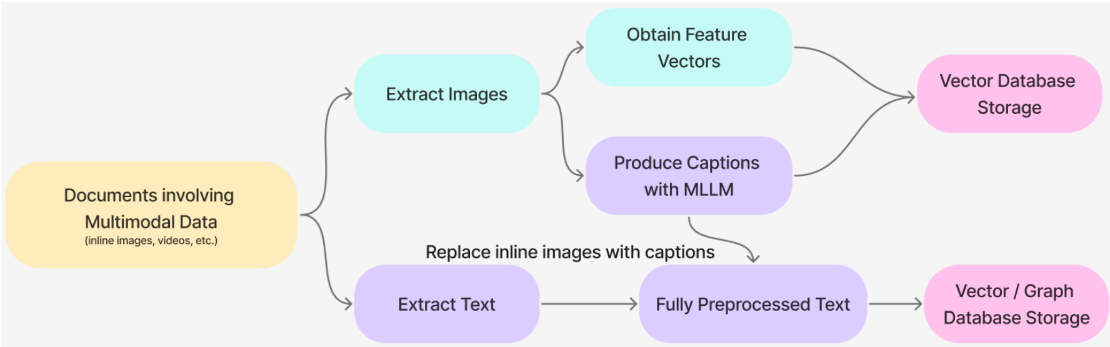
\includegraphics[width=0.8\textwidth]{images/2-method/embedding-flow.png}
            \caption{Flow of embedding and storing documents}
        \end{figure}
    \end{frame}

    \begin{frame}
        \frametitle{Retrieval and Generation}
        Query enhancement using the \textbf{Hypothetical Document Embedding (HyDE)} method:
        \begin{itemize}
            \item Generate a \textbf{zero-shot answer} to the raw user query
            \item Embed and use the zero-shot output for retrieval
            \item Zero-shot answer contains semantic nuances and text patterns of expected document chunks
        \end{itemize}
        However, ablation test results show no significant advantage.
        Left as a configurable option.
    \end{frame}

    \begin{frame}
        \frametitle{Retrieval and Generation}
        Queries to a MLLM may be text-only, or involve text and images.
        \begin{itemize}
            \item \textbf{Text-to-text search}: retrieve similar text chunks by text embedding vector cosine similarity
            \item \textbf{Image-to-image search}: obtain DINOv2 features for query images if present, retrieve similar images by feature vector cosine similarity
            \item \textbf{Text-to-image search}: embed query text into DINOv2 feature space using Talk2DINO, retrieve images by cosine similarity
        \end{itemize}
        Talk2DINO uses the vanilla CLIP text encoder with a limited context size of 77 tokens.
        We use Long-CLIP before the Talk2DINO projection layer for longer context of up to 248 tokens.
    \end{frame}

    \begin{frame}[fragile]
        \frametitle{Retrieval and Generation}
        Top $k$ retrieved document chunks and images are used as context in generation.

        \begin{figure}[H]
            \centering
            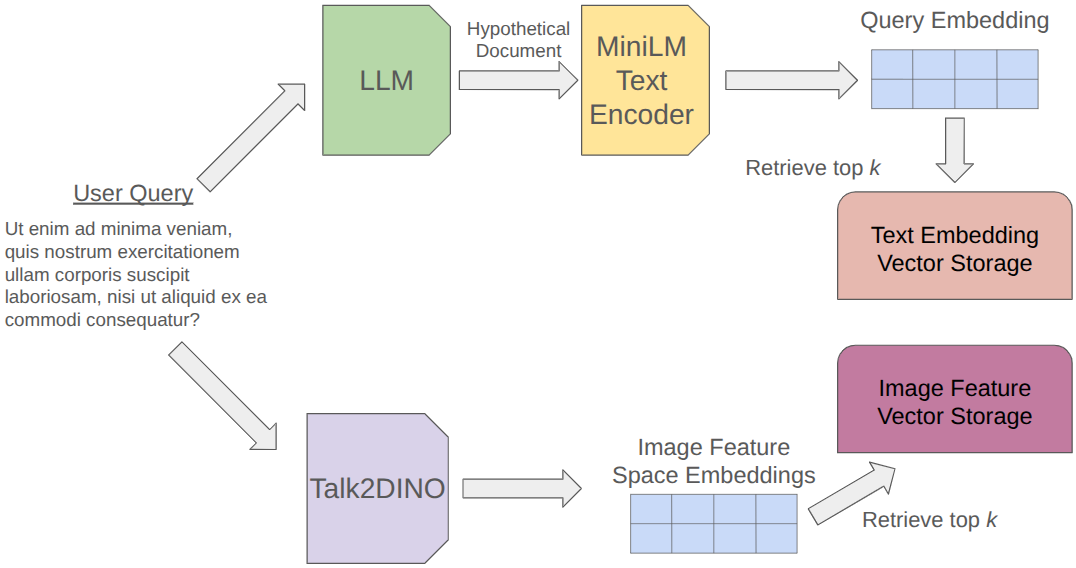
\includegraphics[width=0.7\textwidth]{images/2-method/retrieval-concept.png}
            \caption{Retrieval by text-to-text and text-to-image}
        \end{figure}
    \end{frame}

    \begin{frame}
        \frametitle{Retrieval and Generation}
        When graph storage option is used, text-to-text retrieval goes through the following steps:
        \begin{itemize}
            \item Embed query with MiniLM text embedding model
            \item Embed community summaries with MiniLM text embedding model
            \item Compare relevance of community using embedding vector cosine similarity
        \end{itemize}
        The community summaries of top $k$ most relevant communities are used as retrieved context in generation.
    \end{frame}

    \section{Testing and Evaluation}
    \begin{frame}
        \frametitle{Outline}
        \tableofcontents[currentsection, subsectionstyle=show/shaded] 
    \end{frame}

    \begin{frame}
        \frametitle{Testing}
        We perform a small-scale test on a corpus of 4 documents retrieved from Wikipedia.
        We obtain zero-shot, text-only retrieval, and multimodal retrieval accuracy scores using GPT-4o-mini.

        \begin{itemize}
            \item The level of accuracy increases from zero-shot to text-only retrieval, then multimodal retrieval.
            \item The highest accuracy score is at $k$=7 and 10 under multimodal retrieval.
        \end{itemize}

        This verifies that retrieval benefits answer generation.
    \end{frame}

    \begin{frame}
        \frametitle{Test Example}
        The following is a screenshot taken from an example document in our test corpus.
        \begin{figure}
            \centering
            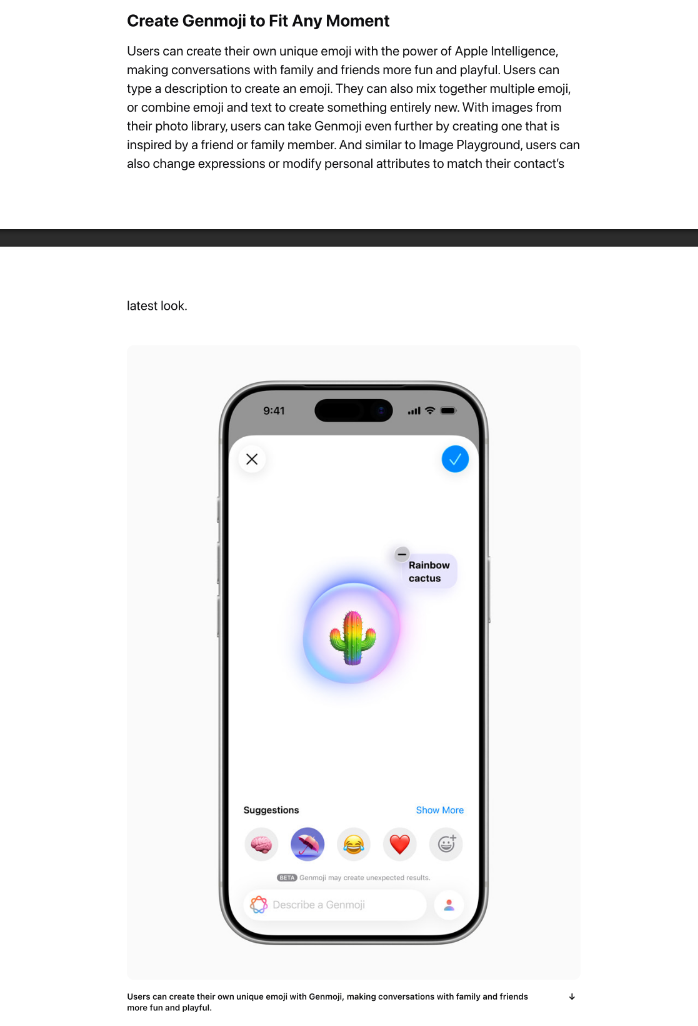
\includegraphics[width=0.28\textwidth]{images/2-method/document-example.png}
            \caption{Part of a document from the test corpus}
        \end{figure}
    \end{frame}

    \begin{frame}[fragile]
        \frametitle{Test Example}
        For the question:
        \footnotesize
        \begin{verbatim}
What is Genmoji like and how can I use it? Can you give me an example?
        \end{verbatim}
        \normalsize

        \begin{columns}[T, onlytextwidth]
            \begin{column}{0.31\textwidth}
                \textbf{Multimodal}\\\smallskip
                \footnotesize
                \texttt{...\\For example, you can create a "rainbow cactus" emoji by describing it, and then you can further customize it by ...}
            \end{column}
            
            \begin{column}{0.31\textwidth}
                \textbf{Text-only}\\\smallskip
                \footnotesize
                \texttt{...\\For example, if you wanted to create an emoji inspired by your friend who loves cats, you might start by ...}
            \end{column}
            
            \begin{column}{0.31\textwidth}
                \textbf{Zero-shot}\\\smallskip
                \footnotesize
                \texttt{1. Access the Platform: Visit the Genmoji website or app. \\ 2. Select Options: Choose facial expressions, accessories, hairstyles...}
            \end{column}
        \end{columns}
        \vspace{2mm}
        
        \normalsize
        Multimodal retrieval mode uses the ``rainbow cactus'' visual context, while text-only retrieval cannot.
        We also see hallucinations in the zero-shot answer, such as a non-existent ``website''.
    \end{frame}

    \begin{frame}
        \frametitle{Benchmarking on MMDocRAG}
        MMDocRAG is a document retrieval and generation benchmark with a dataset of 222 long documents and 4,055 expert-verified QA pairs.
        
        Our results for \textbf{text-only retrieval} are as follows.
        \begin{tabularx}{\textwidth}{@{} c | c c @{}}
            \toprule
            Model & GPT-4o-mini & Qwen2.5VL \\
            \midrule
            \endhead
            \multicolumn{3}{c}{Pure-text input sequence to MLLM} \\
            \midrule
            Zero-shot (no retrieval) & 49.9 (--) & 69.2 (--) \\
            \midrule
            5 quotes (Top-$k$, $k$=5) & 50.4 (--) & 59.6 (--) \\
            7 quotes (Top-$k$, $k$=7) & 51.1 (--) & 59.8 (--) \\
            10 quotes (Top-$k$, $k$=10) & 54.0 (--) & 61.0 (--) \\
            15 quotes (Top-$k$, $k$=15) & 56.9 (70.0) & 61.8 (61.2) \\
            20 quotes (Top-$k$, $k$=20) & \textbf{57.4} (69.8) & \textbf{62.0} (61.4) \\
            \bottomrule
        \end{tabularx}
    \end{frame}

    \begin{frame}
        \frametitle{Benchmarking on MMDocRAG}
        MMDocRAG is a document retrieval and generation benchmark with a dataset of 222 long documents and 4,055 expert-verified QA pairs.
        
        Our results for \textbf{multimodal retrieval} are as follows.
        \begin{tabularx}{\textwidth}{@{} c | c c @{}}
            \toprule
            Model & GPT-4o-mini & Qwen2.5VL \\
            \midrule
            \endhead
            \multicolumn{3}{c}{Pure-text input sequence to MLLM} \\
            \midrule
            Zero-shot (no retrieval) & 49.9 (--) & 69.2 (--) \\
            \midrule
            \multicolumn{3}{c}{Multimodal input sequence to MLLM} \\
            \midrule
            5 quotes (Top-$k$, $k$=5) & 52.7 (--) & 65.8 (--) \\
            7 quotes (Top-$k$, $k$=7) & 55.6 (--) & 66.4 (--) \\
            10 quotes (Top-$k$, $k$=10) & 55.6 (--) & \textbf{67.0} (--) \\
            15 quotes (Top-$k$, $k$=15) & \textbf{57.5} (66.7) & 66.4 (63.2) \\
            20 quotes (Top-$k$, $k$=20) & 55.5 (64.6) & 65.8 (62.6) \\
            \bottomrule
        \end{tabularx}
    \end{frame}

    \begin{frame}
        \frametitle{Benchmarking on MMDocRAG}
        \begin{itemize}
            \item GPT-4o-mini lags behind, while Qwen2.5VL outperforms original paper
            \item Possibly due to performance differences between Azure-provided and OpenAI models
            \item Factuality scores show increasing trend with larger $k$
        \end{itemize}
    \end{frame}

    \begin{frame}
        \frametitle{Benchmarking on Visual-RAG}
        Visual-RAG is based on the iNaturalist 2021 Competition training dataset of 2.7M images of 10,000 biological species.
        Due to time and compute limits, we use the test dataset of 100,000 images to simulate this experiment.

        Results for end-to-end generation are as follows.
        \begin{tabularx}{\textwidth}{@{} c | c c @{}}
            \toprule
            Model & GPT-4o-mini (GPT-4o) & Qwen2.5VL \\
            \midrule
            \endhead
            Zero-shot (no image) & 43.05 (49.33) & 56.68 (34.84) \\
            \midrule
            Top-$k$, $k$=1 & 7.49 (22.65) & 37.43 (37.96) \\
            Top-$k$, $k$=3 & 11.76 (38.50) & 33.42 (39.44) \\
            Top-$k$, $k$=5 & 15.24 (43.45) & 39.57 (39.84) \\
            Top-$k$, $k$=7 & 14.44 (46.52) & 40.91 (38.99) \\
            Top-$k$, $k$=10 & 17.11 (46.93) & 42.25 (42.91) \\
            Top-$k$, $k$=15 & \textbf{19.25} (47.33) & \textbf{46.79} (42.78) \\
            Top-$k$, $k$=20 & 17.91 (50.00) & 43.58 (43.44) \\
            \bottomrule
        \end{tabularx}
    \end{frame}

    \begin{frame}
        \frametitle{Benchmarking on Visual-RAG}
        We further analyze retrieval logs from end-to-end generation experiments, 
        and use the following metrics to evaluate retrieval.
        \begin{itemize}
            \item Recall @$k$: fraction of ground truth images among the top $k$ retrieved images
            \item Normalized Discounted Cumulative Gain (NDCG) @$k$: ranking quality (rewards correct images with higher ranking,
                    discounts relevance logarithmically with position)
            \item Hit @$k$: probability of at least one clue image among the top $k$ images
            \item Hit Count @$k$: number of clue images found in the top $k$ retrieved images
        \end{itemize}
    \end{frame}

    % \begin{frame}
    %     \frametitle{Benchmarking on Visual-RAG}
    %     \begin{tabularx}{\textwidth}{ l | r r r r r r }
    %         \toprule
    %         \textbf{Recall} & @1 & @5 & @7 & @10 & @15 & @20 \\
    %         \midrule
    %         Ours & 3.40 & \textbf{18.37} & 22.75 & \textbf{25.29} & 28.13 & \textbf{30.43} \\
    %         CLIP & 2.81 & 10.26 & -- & 16.70 & -- & 25.54 \\
    %         BGE & \textbf{3.63} & 12.43 & -- & 18.81 & -- & 28.64 \\
    %         VLM2Vec & 2.91 & 10.01 & -- & 16.03 & -- & 26.37 \\
    %         \bottomrule
    %     \end{tabularx}

    %     \begin{tabularx}{\textwidth}{ l | r r r r r r }
    %         \toprule
    %         \textbf{NDCG} & @1 & @5 & @7 & @10 & @15 & @20 \\
    %         \midrule
    %         Ours & \textbf{33.96} & \textbf{35.58} & 31.44 & 22.16 & 21.93 & 22.07 \\
    %         CLIP & 24.33 & 25.97 & -- & 30.98 & -- & 39.21 \\
    %         BGE & 26.74 & 29.15 & -- & \textbf{33.4} & -- & \textbf{41.83} \\
    %         VLM2Vec & 24.87 & 26.33 & -- & 30.09 & -- & 39.13 \\
    %         \bottomrule
    %     \end{tabularx}
    % \end{frame}
    
    % \begin{frame}
    %     \frametitle{Benchmarking on Visual-RAG}
    %     \begin{tabularx}{\textwidth}{ l | r r r r r r }
    %         \toprule
    %         \textbf{Hit} & @1 & @5 & @7 & @10 & @15 & @20 \\
    %         \midrule
    %         Ours & \textbf{33.96} & \textbf{70.86} & 70.86 & \textbf{70.86} & 76.47 & 76.47 \\
    %         CLIP & 24.33 & 53.74 & -- & 67.65 & -- & 77.54 \\
    %         BGE & 26.74 & 58.56 & -- & 68.98 & -- & \textbf{79.14} \\
    %         VLM2Vec & 24.87 & 51.87 & -- & 62.83 & -- & 78.34 \\
    %         \bottomrule
    %     \end{tabularx}

    %     \begin{tabularx}{\textwidth}{ l | r r r r r r }
    %         \toprule
    %         \textbf{Hit Count} & @1 & @5 & @7 & @10 & @15 & @20 \\
    %         \midrule
    %         Ours & \textbf{0.34} & \textbf{1.84} & 2.28 & \textbf{2.53} & 2.81 & 3.04 \\
    %         CLIP & 0.24 & 1.01 & -- & 1.84 & -- & 3.18 \\
    %         BGE & 0.27 & 1.17 & -- & 2.04 & -- & \textbf{3.43} \\
    %         VLM2Vec & 0.25 & 1.10 & -- & 1.91 & -- & 3.33 \\
    %         \bottomrule
    %     \end{tabularx}
    % \end{frame}

    \begin{frame}
        \frametitle{Benchmarking on Visual-RAG}
        Our experiment conditions for retrieval analysis are slightly different from the original paper.
        \begin{itemize}
            \item For retrieval evaluation, the original paper authors select 200-300 images per query
            \item We perform retrieval among all 100,000 images in the test set, making our experiment more difficult for the retriever
        \end{itemize}

        Our results still outperform the original paper in most settings despite the increased difficulty.
        \begin{itemize}
            \item Recall @$k$, Hit @$k$, and Hit Count @$k$ remain higher than other methods in the paper
            \item NDCG values decline for $k > 5$ due to limited number of ground truth images
        \end{itemize}
        These results suggest that our pipeline allows minor fine-grained details to be considered in retrieval.
    \end{frame}

    \begin{frame}
        \frametitle{Additional Note on Benchmark Results}
        Zero-shot generation with Qwen outperforms generation with retrieval, but GPT-4o-mini follows the expected trend.
        \begin{itemize}
            \item Post-training with Supervised Fine-Tuning (SFT) on Qwen2.5 gives long-context generation and logical reasoning
            \item Longer zero-shot answers have higher chance of hitting factual points
            \item LLM judge may award more points as a result
            \item Generation with retrieval does not benefit from model characteristics, model prompted to strictly generate based on retrieved context
        \end{itemize}
    \end{frame}

    \begin{frame}
        \frametitle{Ablation Test: CLIP vs DINOv2}
        We perform an ablation test on using CLIP for embedding images and multimodal retrieval on GPT-4o-mini.
        \begin{itemize}
            \item Our DINOv2-Talk2DINO pipeline achieves higher accuracy for $k$=1, 3, 7, 10 compared to CLIP
            \item The highest accuracy is from using the DINOv2-Talk2DINO pipeline
            \item CLIP underpeforms DINOv2 in most settings
            \item Unified representation space for text and vision in CLIP loses fine-grained details
            \item Results validate the dual representation design for multimodal processing
        \end{itemize}
    \end{frame}

    \begin{frame}
        \frametitle{Ablation Test: HyDE}
        We perform experiments to compare accuracy between using HyDE or raw query embeddings for dense retrieval.
        \begin{itemize}
            \item HyDE won in 8, raw query in 5, and 1 tie
            \item No clear trend with respect to $k$ observed
            \item Adds additional computation cost in generating the hypothetical document
        \end{itemize}

        Our results do not lead to a clear conclusion on which method is better.
        We leave this as a configurable option.
    \end{frame}

    \section{Discussion}
    \begin{frame}
        \frametitle{Outline}
        \tableofcontents[currentsection, subsectionstyle=show/shaded] 
    \end{frame}

    \begin{frame}
        \frametitle{Analysis of Findings}
        We find the following issues in analyzing failure cases.
        \begin{itemize}
            \item Multi-column document comprehension errors causes noise in embedding and retrieval
            \item Knowledge graph option retrieves context using flattened community summaries, loses specific details
            \item More retrieved text benefits end-to-end generation accuracy, but too much visual context may harm generation
                \begin{itemize}
                    \item Visual retrieval provides fine-grained visual information for answering questions
                    \item Large batches of images may introduce noise and confuse the MLLM
                \end{itemize}
        \end{itemize}
    \end{frame}

    \begin{frame}
        \frametitle{Limitations}
        \begin{itemize}
            \item Preprocessing overhead and limitations
                \begin{itemize}
                    \item Using MLLM for image captioning incurs an overhead of average 3.89 seconds per image
                    \item Video processing not included in our pipeline
                \end{itemize}
            \item Dense retrieval theoretical limits
                \begin{itemize}
                    \item Theoretical limits in retrieval effectiveness with respect to the number of documents to store, the number of items to retrieve, and dense vector dimensionality
                    \item Corporate-grade applications with hundreds to thousands of documents may reach such limits
                \end{itemize}
            \item MLLM perception lacking behind human vision
                \begin{itemize}
                    \item Pipeline based on assumption that relevant images provide visual evidence to further ground generation
                    \item Current MLLMs show severe deficits in visual perception without textual fallback
                    \item Severe lack in MLLM capability when visual content cannot be translated into natural language
                \end{itemize}
        \end{itemize}
    \end{frame}

    \begin{frame}
        \frametitle{Future Work}
        \begin{itemize}
            \item Better preprocessing efficiency, such as by parallel MLLM calls for captioning
            \item Fine-tuning foundation models (DINOv2, Talk2DINO) for specific domain applications
            \item Retrieval methods: agentic retrieval for better flexibility, rerankers to sort top-$k$ retrieved items
            \item Further research on improving MLLM visual perception capabilities
            \item Application to text-to-vision models for better use of retrieved visual details
        \end{itemize}
    \end{frame}

    \section{Conclusion}
    \begin{frame}
        \frametitle{Outline}
        \tableofcontents[currentsection, subsectionstyle=show/shaded] 
    \end{frame}

    \begin{frame}
        \frametitle{Conclusion}
        We present a multimodal Retrieval-Augmented Generation (RAG) pipeline in this thesis, with a focus on visual elements.
        \begin{itemize}
            \item We provide a complete pipeline that supports text and text-image queries, with evidence covering both modalities;
            \item We utilize state-of-the-art pretrained foundational models (DINOv2, Talk2DINO), a method without fine-tuning requirements;
            \item We achieve results on par with or slightly better than existing methods on research benchmarks.
        \end{itemize}

        Despite limitations in preprocessing and MLLM perception, our pipeline offers a foundation for grounding MLLM generation with retrieved visual evidence.

        Future work will explore better preprocessing efficiency, agentic retrieval and reranking, domain-specific fine-tuning, and extension to application with text-to-vision models.
    \end{frame}

    \begin{frame}{Thank you}
        \begin{center}
            \Huge \textbf{Thank you!} \\[1cm]
            \Large \textbf{Questions?} \\[1.5cm]
        \end{center}
    \end{frame}

\end{document}